\section{Analysis}
%\subsection{Comparing text of the tweet and document}

This section details the analyses performed on the data. The analyses mimic the ROUGE-1,2 and L methods of comparing documents, where we compare the tweet and article text using these methods. This is done to determine whether the tweets promoting the articles could be generated from the document text. The results of the comparison show that the tweet is not extracted from the article text. 

We calculate the degree of common words - unigrams and bigrams, between the tweet and the text of the document. We also check least common subsequences between the tweet and the document. These are the ROUGE-1,2 and L methods. The hypothesis is that these results give an approximation of the degree to which the tweet is extracted from the document text. 

For all these analyses, the stop words have been eliminated from the tweet as well as the document, so that only the significant words are taken into consideration. The hastags, references (@) and URLs from the tweets were also all removed.

\subsection {Total match with text in article}

To calculate the position of tweet text as a whole in the text, we checked for a complete substring match of the tweet in the text. Out of the 2471 unique instances of tweet text and the article text pairs, where a tweet text was checked against the text in the article, a complete match was found 23 times. 9 times out of these, the tweet text had been matched against the title of the article extracted into the text. The rest of the results are significant, since the text of the tweet appears exactly as is inside the text of the article. For these cases, the user that wrote the tweet went through the article text, and the sentence that either seemed to be the most conclusive contribution of the article, or expressed the opinion of the user was extracted to be tweeted. We also checked to see if the tweet text matched with the article titles, and this was found not to be the case. 

Overall, this comparison showed that if the tweet is extracted as a whole from the document, it is either from the title, or actually from inside the document text that was found most appropriate by the user. 

\subsection{Percentage match for unigrams}

Next, we did a percentage match with the text of the article. This was a bag-of-words check using unigrams from the tweet and the document. The order of the words in the tweet or the text did not matter. The results we got seem to suggest that a lot of significant words in the tweet are in fact present in the article. The minimum percentage match obtained was 60\%. However, since the order of the words did not matter, this result can  be traced back to the fact that tweet is based on the same topic as the document. \figref{fig:unigrammatch} shows the percentage of matches in the tweet and the article text as compared to the number of unigrams in the tweet. The mean of the match percentages is 29.53 and standard deviation is 20.2. \improvement{Add and #words matching}

\begin{equation}
\resizebox{.9\hsize}{!}{$unigramMatch = \frac{| unigrams(tweet) \cap unigrams(text) |}{| unigrams(tweet) |} * 100$}
\end{equation}

\begin{figure}[htbp]
\centering
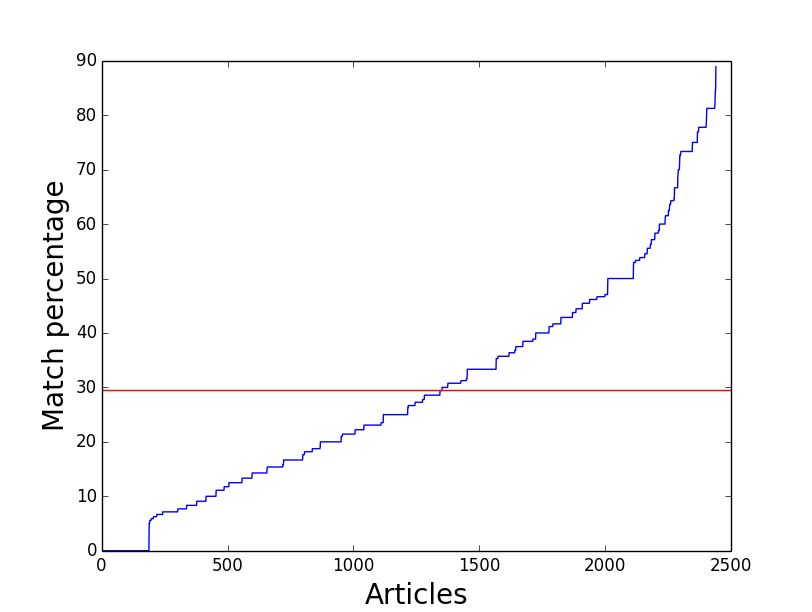
\includegraphics[width=0.5\textwidth, height=6cm]{unigrammatch}
\caption{Unigram match percentage.}
\label{fig:unigrammatch}
\end{figure}

\subsection{Percentage match for bigrams}

Similar to the unigram matching techniques, bigram percentage matching was also calculated. The text of the tweet was converted into bigrams and we then looked for those bigrams in the article text. The percentage was calculated similar to the unigram matching done earlier. \improvement{Add #words matching}

\begin{equation}
\resizebox{.9\hsize}{!}{$bigramMatch = \frac{| bigrams(tweet) \cap bigrams(text) |}{| bigrams(tweet) |} * 100$}
\end{equation}

\figref{fig:bigrammatch} shows the percentages of matches found in every article. Mean is 10.73 with a standard deviation of 18.5.

\begin{figure}[htbp]
\centering
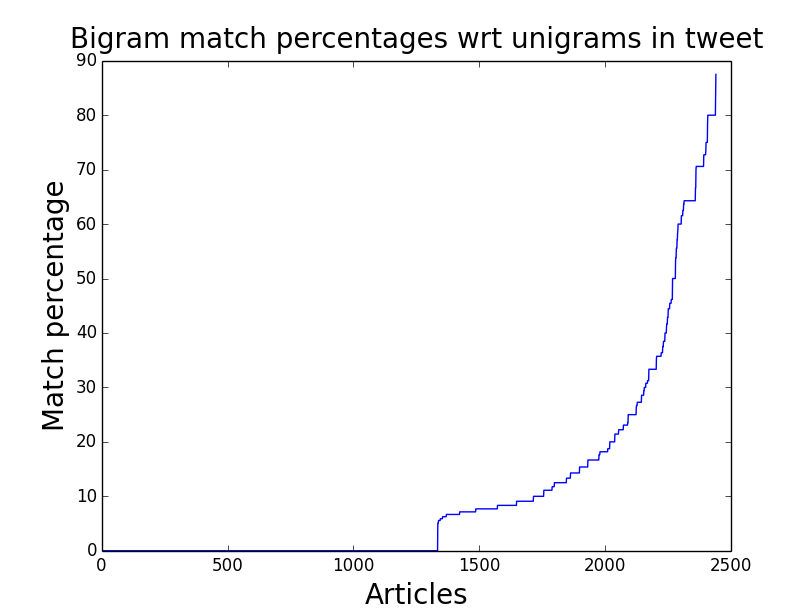
\includegraphics[width=0.5\textwidth, height=6cm]{bigrammatch}
\caption{Bigram match percentage.}
\label{fig:bigrammatch}
\end{figure}

\subsection{Percentage matching inside a window in the article text}

The next analysis was to check for a significant word matching inside a two or three sentence window inside the article text. We used a three sentence long window using the sentence boundary information obtained during preprocessing. After the text of the window was extracted, we performed a similar analysis as the last one, except on a smaller set of sentences. Again, the order of the unigrams didn't matter. Next, the matching percentages from all such windows in the articles were compared and the maximum out of these was considered for the highest match percentage and match position for the final results. The result from this experiment is shown in \figref{fig:unigramwindow}. Here, the mean of the values is 26.6\% and deviation 17\%.\improvement(Add equation for this matching)\improvement{Add position and #words matching}

\begin{figure}[htbp]
\centering
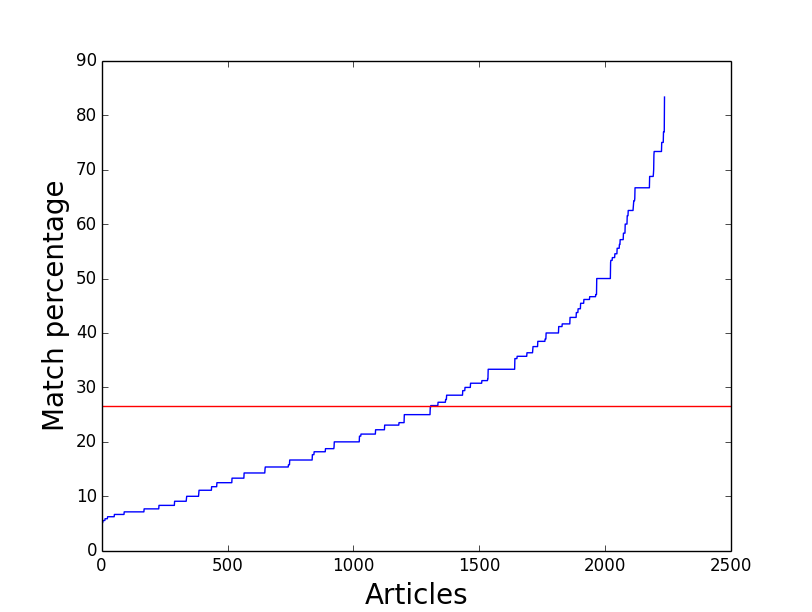
\includegraphics[width=0.5\textwidth, height=6cm]{unigramwindow}
\caption{Percentages of common words in tweet and text.}
\label{fig:unigramwindow}
\end{figure}

\subsection{Longest Common Subsequence match inside a window for the text}

The percentage match analyses were a bag-of-words approach disregarding the order of the words inside the texts and tweets. To respect the order of the words in the sentence of the tweet, we also used the least common subsequence algorithm between the tweet text and the document text. This subsequence matching was done inside a sentence window of 5 sentences. Again, the final result for the article was the window in which the maximum percentage was recorded among all windows. The percentage match was calculated against the number of words in the tweet, as found in the least common subsequence calculated between the two texts. These numbers are shown in \figref{fig:lcs}. The mean here is 44.6\% and the standard deviation is 22.7\%. \improvement{change graph to reflect positions}

\begin{equation}
\resizebox{.9\hsize}{!}{$LCSMatch = \frac{| lcs(tweet, text) |}{| unigrams(tweet) |} * 100$}
\end{equation}

\begin{figure}[htbp]
\centering
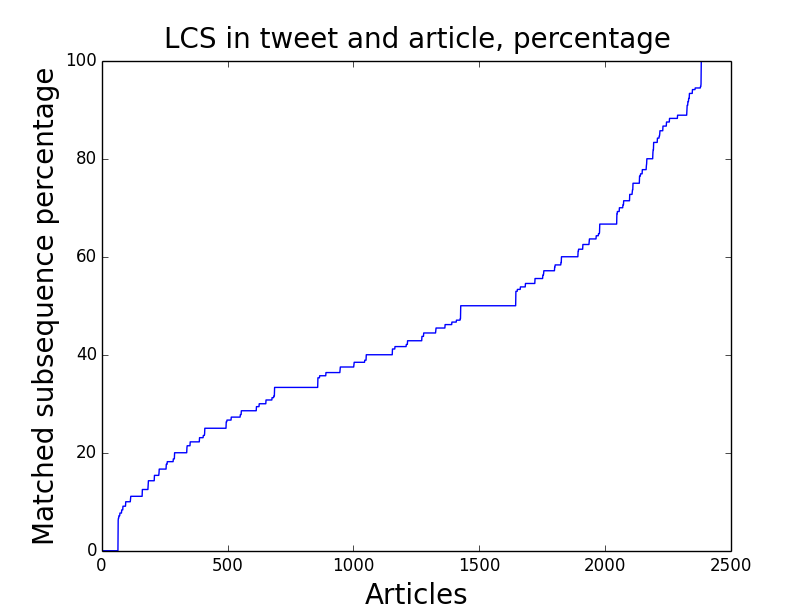
\includegraphics[width=0.5\textwidth, height=6cm]{lcs_doc}
\caption{Percentages of words matching in tweet and document text using an LCS algorithm.}
\label{fig:lcs}
\end{figure}


% \subsection{Subjectivity and Formality}
% \change{should subjectivity be included?}

